\documentclass{article}

\usepackage[spanish]{babel}
\usepackage[numbers,sort&compress]{natbib}
\usepackage{graphicx}
\usepackage{subfigure}
\usepackage{url}
\usepackage{amsmath}
\usepackage{hyperref}
\usepackage[top=15mm, bottom=40mm, left=15mm, right=15mm]{geometry}
\setlength{\parskip}{2mm}
\setlength{\parindent}{0pt}



\author{Dulce Esperanza Carrasco Castillo 1445183}
\title{Práctica 3: Teoría de colas}
\date{\today}

\begin{document}

\maketitle

\section{Objetivo}
Conocer que la rapidez de ejecución de tareas en paralelo depende de la cantidad de núcleos que realmente están trabajando y también del orden en el que se estén ejecutando las tareas.

\section{Descripción}
En esta práctica se midió el tiempo que se tarda realizar ciertas tareas, se utilizó la combinación de números primos y no primos en diferente proporción y se varió la cantidad de núcleos trabajando. 
Primero se verificó la cantidad de núcleos con los que cuenta el dispositivo en el que se trabajó usando el comando: detectCores(), se creó un vector para los números primos y otro para los números no primos (misma cantidad de números de cada uno) \ref{codigo}, después se hizo otro vector para combinar los números primos y no primos y que tomara los números aleatoriamente. Para variar la proporción se disminuía la cantidad de números a un vector(primos) y se le agregaban al otro(noprimos) para mantener la misma cantidad de números totales. Se corrieron para 3,2 y 1 núcleo. Se repitió el proceso para números de 7 y 9 dígitos. 
 

\section{Resultados}

Se observa en la figura \ref{figura 1} que al usar la mayor cantidad de núcleos los tiempos de ejecución no varían mucho pero si se lleva más tiempo cuando está en una proporción 50/50, de manera que al disminuir la cantidad de primos o noprimos disminuye el tiempo de ejecución. Con dos núcleos, el trabajo se reparte de manera más ordenada y con un núcleo se puede ver que los números primos hacen la tarea más pesada.

En la figura \ref{figura 2} se utilizan números de 7 dígitos, se puede observar que al usar la mayor cantidad de núcleos los tiempos de ejecución son menores y va aumentando conforme se usan menos núcleos para realizar la tarea. Al usar menor cantidad de núcleos los números primos hacen la tarea más pesada y el tiempo de ejecución es mayor.

En la figura \ref{figura 3} se utilizaron números con 9 dígitos, se puede ver que los tiempos son más grandes que los tiempos con 5 y 7 dígitos, y hay mucha diferencia entre los tiempos que se tarda cada combinación, lo que vuelve a confirmar que donde hay mayor cantidad de números primos, mayor es el tiempo que se tarda en realizar la tarea, por lo que los números primos hacen la tarea pesada. 


\begin{figure}
\centering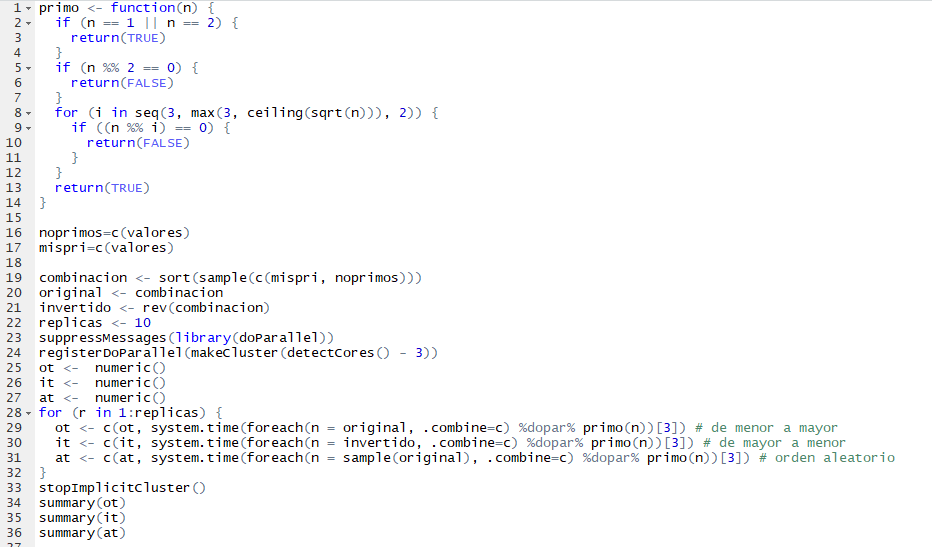
\includegraphics[width=120mm]{codigo.png}
\caption{Código}
\label{codigo}
\end{figure}

\begin{figure}[htbp]
\centering
\subfigure[]{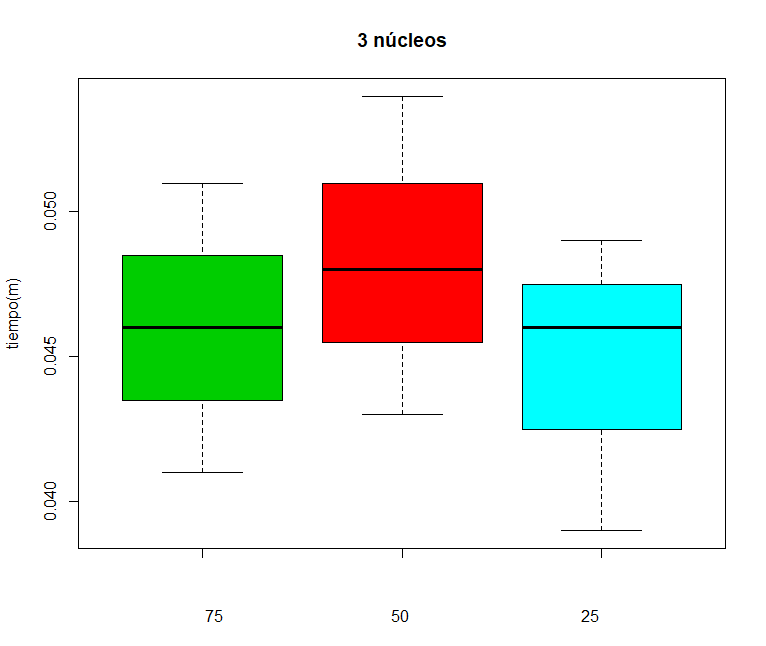
\includegraphics[width=60mm]{./3nucleos5.png}}
\subfigure[]{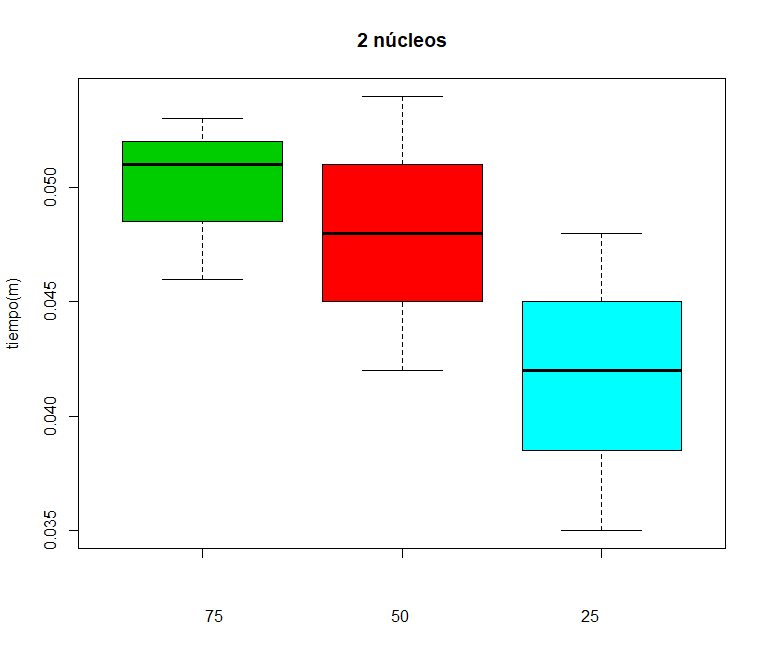
\includegraphics[width=60mm]{./2nucleos5.png}}
\subfigure[]{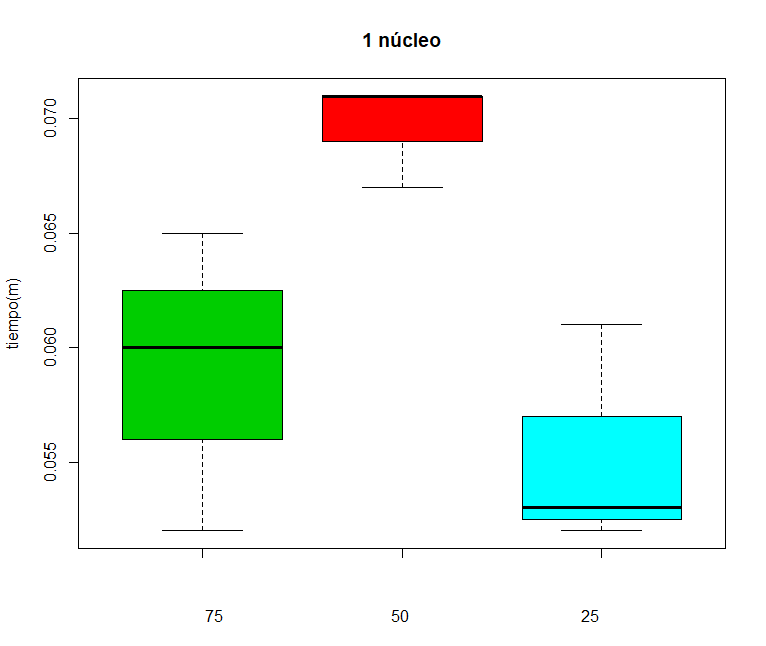
\includegraphics[width=60mm]{./1nucleo5.png}}
\caption{5 dígitos} \label{figura 1}
\end{figure}

\begin{figure}[htbp]
\centering
\subfigure[]{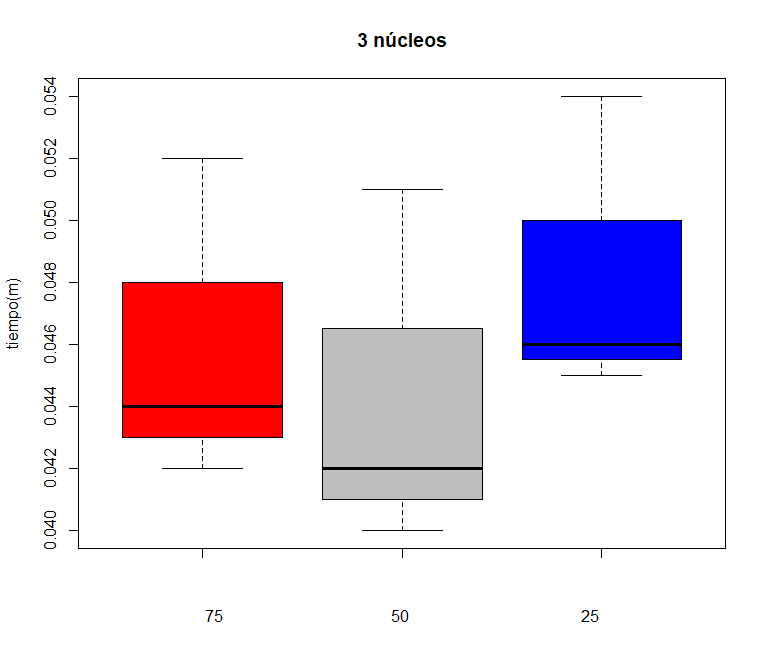
\includegraphics[width=60mm]{./3nucleos7.png}}
\subfigure[]{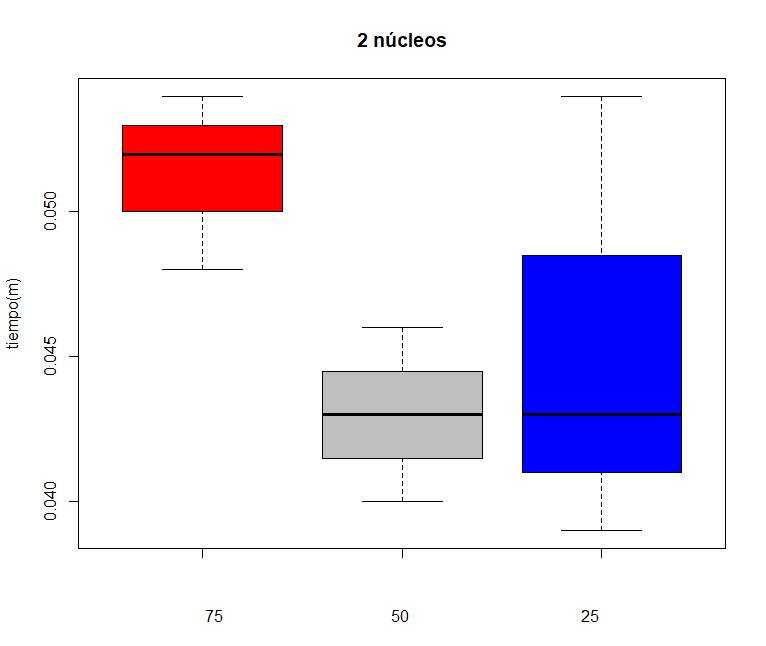
\includegraphics[width=60mm]{./2nucleos7.png}}
\subfigure[]{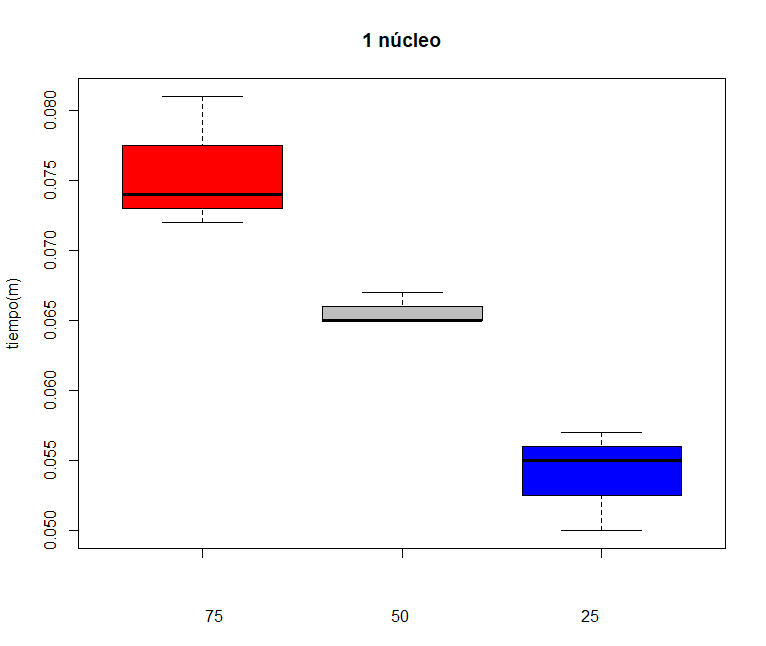
\includegraphics[width=60mm]{./1nucleo7.png}}
\caption{7 dígitos} \label{figura 2}
\end{figure}

\begin{figure}[htbp]
\centering
\subfigure[]{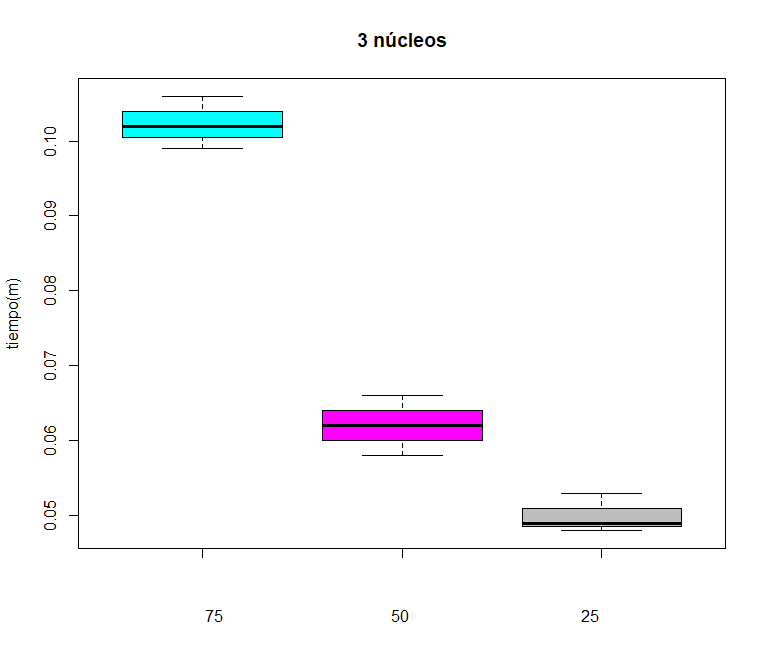
\includegraphics[width=60mm]{./3nucleos9.png}}
\subfigure[]{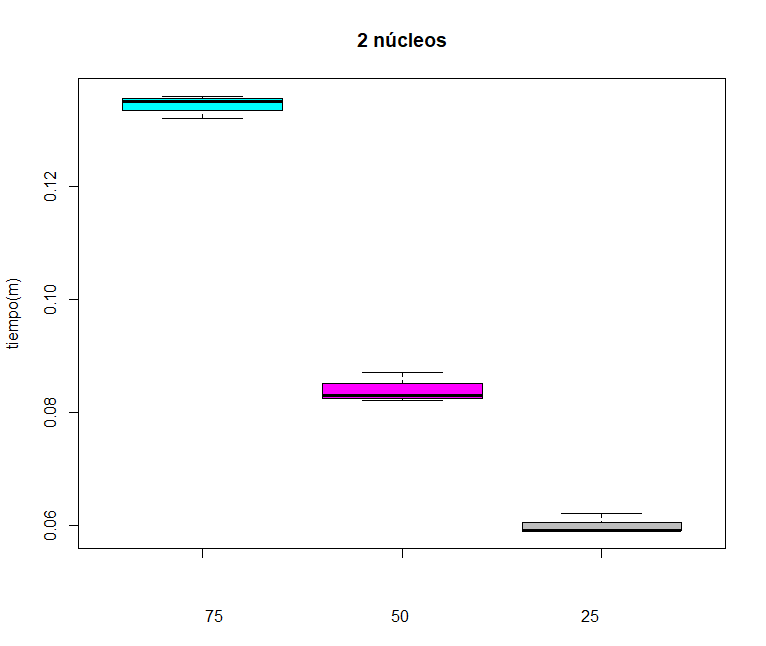
\includegraphics[width=60mm]{./2nucleos9.png}}
\subfigure[]{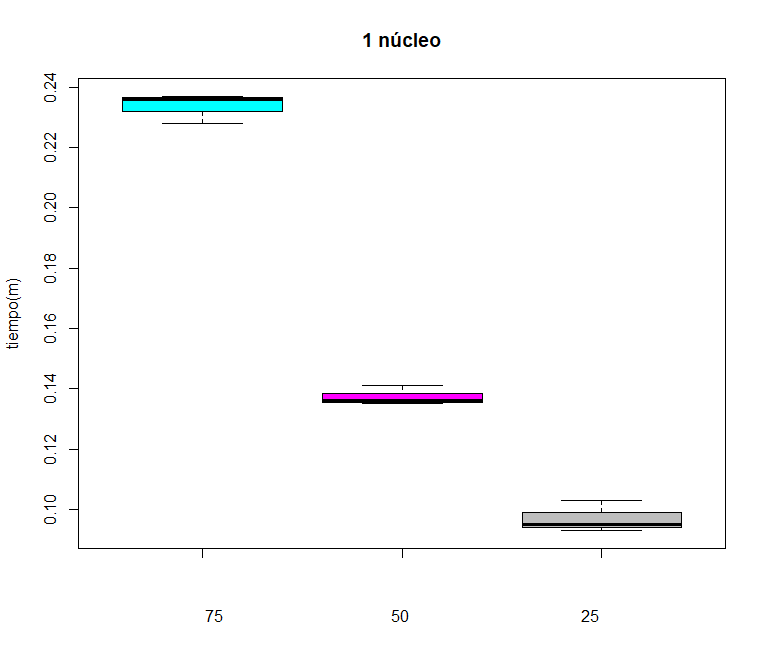
\includegraphics[width=60mm]{./1nucleo9.png}}
\caption{9 dígitos} \label{figura 3}
\end{figure}

\newpage

\bibliographystyle{plainnat}
\bibliography{Bibliosimu}

\end{document}